\section{Method}

\subsection{Singularity}
A Singularity image needs a so called "receipt", which is a file that tells Singularity how to create the image and what to include in it. The recipe was added to Singularity Hub, a library were Singularity receipts can be uploaded, then built and shared with other users \cite{singularity-hub}.

To complete the workflow from raw data to protein quantification results, several other software than Quandenser had to be included in the container, which are listed below.

\subsubsection{MSconvert}
There exist a multitude of different types of MS data format, which can cause compatibility issues with existing software. The MS format depends on which instrument was used to generate the data, but most software cannot directly use any vendor-specific formatted files, meaning they have to be converted to a general MS data format first, namely files of type mzML \cite{mzml-format}. To combat the problem with incompatible data, a software named \textit{MSconvert} was added to the workflow, which can convert MS data from a multitude of vendor formats to the general MS data format needed to run Quandenser \cite{proteowizard}. Due to conversion from vendor formats with Msconvert only works on Windows operative systems, another solution was needed, since the Singularity image was based on Ubuntu, a Linux operative system. The solution was to use another type of software called \textit{Wine}, which adds an compatibility layer in Portable Operating System Interface (POSIX) systems, which includes Linux, to run Windows software \cite{wine}. The Singularity image was based on another image created by the proteowizard developers, which incorporates all the necessary components to run Wine and MSconvert \cite{docker-image} \cite{docker-howto}.

\subsubsection{Crux}
Crux is an open source mass spectrometry analysis toolkit available for Linux, Windows and MacOS \cite{crux}. The purpose of integrating Crux into the image was to use three specific tools; tide-index, tide-search and percolator. Tide-index is a pre-search tool that adds indexes and decoys to the protein data base, which is used by the search tool tide-search, that parses fragmentation spectra and creates peptide-to-spectrum matches (PSMs) \cite{tide-search}. Percolator is a post-search tool, that separates peptide targets from decoy PSMs \cite{percolator}. In combination, the tools were used to post-process the output from Quandenser to prepare it for the software Triqler, explained in the next section.

\subsubsection{Triqler}
Triqler is an software which uses using graphical models and bayesian statistics to find differentially expressed proteins between samples. The main benefit with using Triqler in combination with Quandenser is that it utilizes both MS2 and MS1 spectra from the files, which improves the overall quantification of proteins \cite{triqler}.

\subsection{Nextflow}

\begin{wrapfigure}{r}{4cm}
  \centering
  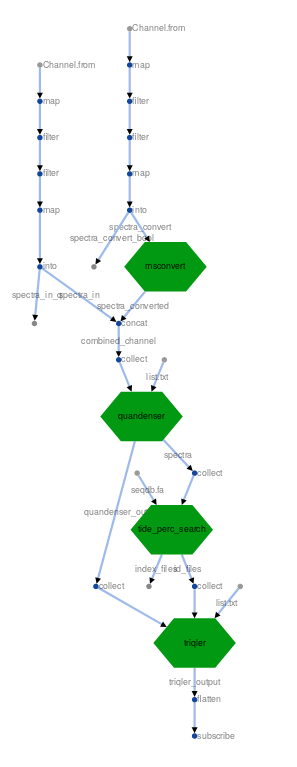
\includegraphics[width=4cm, height=5cm]{pictures/workflow.png}
  \caption{Workflow of the pipeline}
  \label{fig:workflow}
\end{wrapfigure}

Nextflow has integrated compatibility with running software inside Singularity images, which is used to call on the programs contained in the Singularity image. The pipeline is shown in figure \ref{fig:workflow}. Due to Nextflow's capability of running multiple software in parallel, a modified version of Quandenser was added to fully utilize the parallelization. When running the parallelized version of Quandenser in the pipeline, the process is divided into five parts, two of which are parallelizable. The aim was to speed up the calculation time when running large cohorts, since the time scaling of an increased number of files was not a linear relationship to the processing time.

Nextflow also has the benefit of being able to submit processes to workload managers, which are used on HPC clusters to allocate processing time for users. To be able to run the pipeline on HPC clusters, the pipeline is outfitted with an option to enable submitting processes via SLURM, the current workload manager on UPPMAX.


\subsection{Quandenser-pipeline GUI}
To integrate the Singularity image and the Nextflow pipeline, a GUI was created and packed into the image to improve the usability of the workflow, to allow users to easily modify and run the pipeline to their choosing. Pyside2 was used to create the GUI, which is an open source GUI framework based by the Qt framework \cite{pyside2}. A shell script handling installing Singularity, downloading the image from Singularity Hub and starting the GUI inside the image. Figure \ref{fig:GUI_workflow} shows the GUI workflow. The user downloads the shell script and executes it, which installs singularity, downloads the Singularity image, then starts the GUI. The GUI is used to modify the configuration files, which affects how the pipeline is executed. When the user wants to run the pipeline, the GUI communicates to the shell script with a "named pipe", i.e a file which both the GUI and the shell script has access, that tells the shell script to execute the nextflow pipeline. The pipeline loads the configuration files, then calls on the image to execute the programs in the image at a particular order.

\begin{figure}[!htbp]
  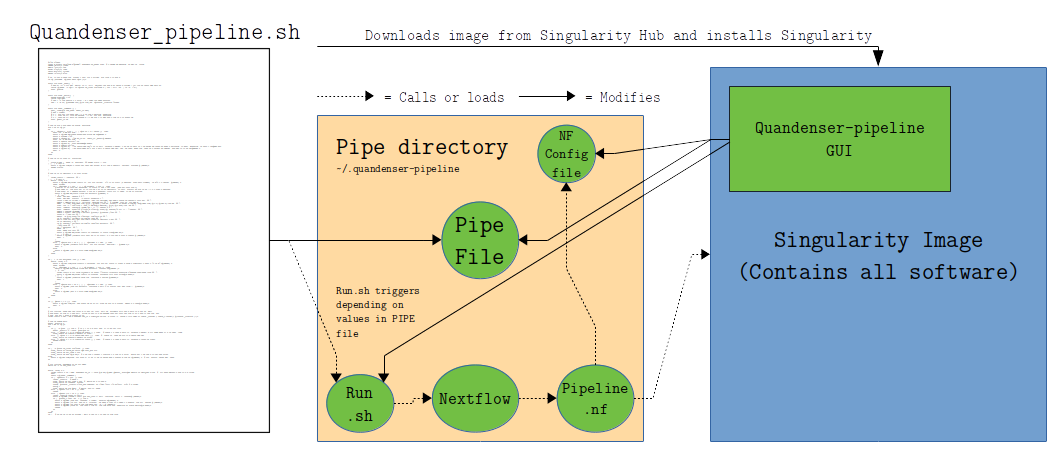
\includegraphics[width=\linewidth]{pictures/GUI_workflow.png}
  \caption{GUI workflow of Quandenser-pipeline}
  \label{fig:GUI_workflow}
\end{figure}


\subsection{Analysing bacterial proteomes}
The RAW data files for the cyanobacteria data set was on average 0.8 Gb in size and ralstonia data set 1.3 Gb. Both data sets were run on different established proteomic pipelines to compare the performance of the newly created pipeline. The following table illustrates which programs were used:

\newcommand{\textone}{\small The pipeline created for the thesis, using Quandenser as it's cornerstone. Due to Singularity not supporting non POSIX systems, the Windows OS cannot run the pipeline natively without using a compatibility layer suggested in the Singularity documentation \cite{singularity-documentation}.}
\newcommand{\texttwo}{\small The custom pipeline tested on the data set was created by the workflow manager \textit{KNIME} in combination with \textit{OpenMS}, creating a custom workflow for analyzing mzML data \cite{knime} \cite{openms}. The pipeline was created by Michael Jahn at SciLifeLab and is used to analyze bacterial data \cite{m-jahn-pipeline}. Both KNIME and OpenMS is available for Linux, MacOS and Windows.}
\newcommand{\textthree}{\small MaxQuant is a tool used for quantitative proteomics and is well suited for analyzing label-free proteomic data. The tool is available for Windows and at also now for Linux, if the Mono framework is used \cite{maxquant} \cite{maxquant-installation}.}
\newcommand{\textfour}{\small MetaMorpheus is a search engine software which can find Post-Translational Modifications Modifications (PTMs) and integrates Flash LFQ, a label-free peptide quantification software into the pipeline \cite{metamorpheus}. MetaMorpheus is only available for the Windows OS.}
\newcommand{\textfive}{\small The Trans-Proteomic Pipeline (TPP) is an open-source proteomics data pipeline which includes a multitude of tools for analyzing proteomic data \cite{TPP}. The pipeline is available for Windows and a Linux distribution called Ubuntu}
\newcommand{\textsix}{\small Philosopher is a proteomics newly created toolkit which is available for multiple types of POSIX systems and Windows, which uses modified software used in the TPP pipeline for analysis \cite{philosopher}.}

\begin{table}[H]
\begin{tabular}{|p{4cm}|p{9cm}|}
\hline
Program & Description \\ \hline \hline
Quandenser-pipeline v0.051 & \textone \\ \hline
KNIME + OpenMS & \texttwo \\ \hline
MaxQuant 1.6.5 & \textthree \\ \hline
MetaMorpheus 0.0.299 & \textfour \\ \hline
Trans-Proteomic Pipeline 5.2.0 & \textfive \\ \hline
Philosopher 20190322 & \textsix \\ \hline
\end{tabular}
\caption{Different pipelines used to compare Quandenser-pipeline}
\end{table}

The pipelines were compared by the time it took to process the data sets, how many proteins were discovered and also how many proteins the pipeline found to be differentially expressed.

To define a differentially expressed protein,


\begin{equation}
E=m
\end{equation}


was defined as any protein which had a q-value less than 0.01 for
